\documentclass[11pt]{article}

\usepackage{subcaption}
\usepackage{graphicx}
\usepackage{amsmath}
\usepackage{relsize}
\usepackage{natbib}
\usepackage{float}
\usepackage[margin=1in]{geometry}
\usepackage{tikz}

\usetikzlibrary{shapes,arrows}

\tikzstyle{block} = [rectangle, draw, thick, align=center, rounded corners]
\tikzstyle{boundingbox} = [very thick, dotted, gray]
\tikzstyle{dashblock} = [rectangle, draw, thick, align=center, dashed]
\tikzstyle{conc} = [ellipse, draw, thick, dashed, align=center]
\tikzstyle{netnode} = [circle, draw, very thick, inner sep=0pt, minimum size=0.5cm]
\tikzstyle{relunode} = [rectangle, draw, very thick, inner sep=0pt, minimum size=0.5cm]
\tikzstyle{line} = [draw, very thick, -latex']

\begin{document}

\section{Introduction}
Humans are able to use and reuse knowledge more flexibly than most deep learning models can \citep{Lake2017}. One fundamental reason for this is the siloing of knowledge within deep neural networks -- although deep networks represent knowledge about data (activations) and knowledge about transformations of that data (parameters), they do not represent any relationships between these. By contrast, humans are (or can be) consciously aware of both our representations of input, the transformations we can perform on them, and the relationships between data and functions on the data. This is true for domains from game playing to natural language understanding. \par
One of the abilities that this grants humans is the ability to learn rapidly from relatively few examples. This problem has been partially addressed by meta-learning systems \citep{}. Yet humans can then take this knowledge and flexibly alter their behavior in accordance with a change in task demands or a single instruction. For example, once we learn to play a game, we can immediately switch to playing in order to lose, and can achieve reasonable performance \textbf{without any retraining} (i.e. zero-shot). Deep learning systems at present lack this flexiblity. \par
In this paper, we propose a new class of architectures which essentially take a \textbf{functional perspective} on meta-learning. By treating both data and transformations on the data as functions, we can conceptually think of both as transformable data. This yields the ability to not just learn to solve new tasks, but to learn how to flexibly transform these solutions in response to changing task demands. We suggest that this ability will be key to building more intelligent deep learning systems. \par

\section{Method}
We take a \textbf{functional} perspective on learning. A datum can be represented by a constant function which outputs it. (For example, each point in the latent space of an autoencoder can be thought of this way.) This allows us to interpret model inputs or outputs as functions. \par
We can then interpret most machine learning tasks as a mapping of functions to functions. These functions could represent data\footnote{Where ``data'' is a quite flexible term. The approach is relatively agnostic to whether the learning is supervised or reinforcement learning, e.g.}, or they could be functions that operate on functions themselves. Under this perspective, learning tasks and learning to flexibly map between tasks are the same type of problem. \par
Specificially, we 

\begin{figure}
\centering
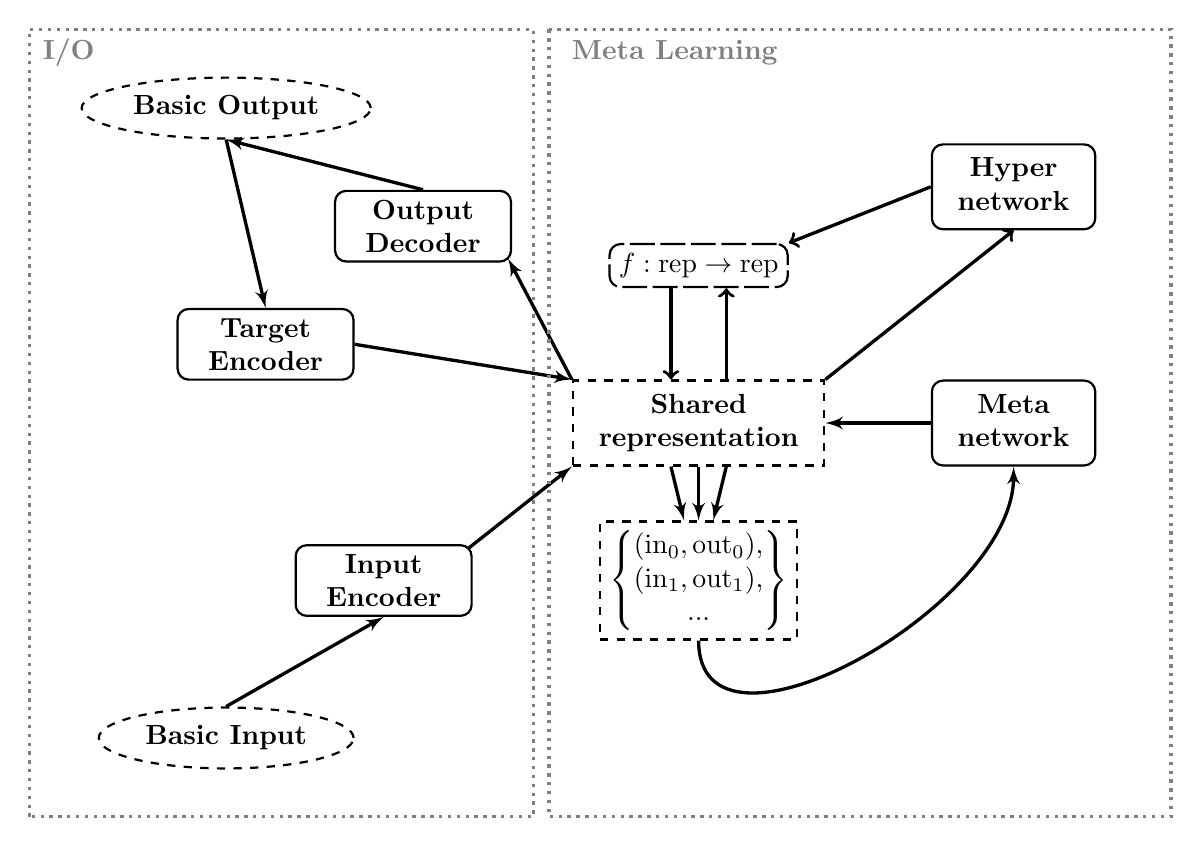
\begin{tikzpicture}[auto]

\node [dashblock] at (0, 0) (rep) {\begin{tabular}{c}\textbf{Shared} \\ \textbf{representation}\end{tabular}};

% inputs, outputs

\draw [boundingbox] (-8.5, -5) rectangle (-2.1, 5); 
\node [text=gray] at (-8, 4.7) {\textbf{I/O}};

\node [conc] at (-6, -4) (perc) {\textbf{Basic Input}};
\node [conc] at (-6, 4) (act) {\textbf{Basic Output}};
\node [block, text width=2cm] at (-4, -2) (IE) {\textbf{Input Encoder}};
\node [block, text width=2cm] at (-3.5, 2.5) (OD) {\textbf{Output Decoder}};
\node [block, text width=2cm] at (-5.5, 1) (TE) {\textbf{Target Encoder}};
\path [line] (perc.north) to (IE.south);
\path [line] ([xshift=-0.05cm, yshift=-0.05cm]IE.north east) to (rep.south west);
\path [line] (rep.north west) to ([xshift=-0.05cm, yshift=0.05cm]OD.south east);
\path [line] (OD.north) to (act.south);
\path [line] (act.south) to (TE.north);
\path [line] (TE.east) to (rep.north west);

% meta
\draw [boundingbox] (-1.9, 5) rectangle (6, -5); 
\node [text=gray] at (-0.3, 4.7) {\textbf{Meta Learning}};

\node [dashblock] at (0, -2) (collection) {
\(\left\{
\begin{matrix}
(\text{in}_0, \text{out}_0),\\
(\text{in}_1, \text{out}_1),\\
...  
\end{matrix}\right\}\)};
\path [line] (rep.south) to (collection);
\path [line] ([xshift=-1em]rep.south) to (collection);
\path [line] ([xshift=1em]rep.south) to (collection);

\node [block] at (4, 0) (meta) {\begin{tabular}{c}\textbf{Meta} \\ \textbf{network}\end{tabular}};
\path [line] (collection.south) to [out=-90, in=-90] (meta.south);
\path [line] (meta.west) to (rep.east);

% hyper

\node [block] at (4, 3) (hyper) {\begin{tabular}{c}\textbf{Hyper} \\ \textbf{network}\end{tabular}};
\node [block, dash pattern=on 9pt off 2pt] at (0, 2) (transform) {\(f: \text{rep} \rightarrow \text{rep}\)};

\path [draw, ->, very thick] (rep.north east) to (hyper.south);
\path [draw, ->, very thick] (hyper.west) to (transform.north east);
\path [draw, ->, very thick] ([xshift=-1em]transform.south) to ([xshift=-1em]rep.north);
\path [draw, ->, very thick] ([xshift=1em]rep.north) to ([xshift=1em]transform.south);

\end{tikzpicture}
\caption{Schematic of our general architecure.}
\end{figure}

\section{Results}

\section{Discussion}

\end{document}

